\subsection*{Experiment 8.01 \quad Measurement of the focal length of a convex lens by three different methods}

\textbf{[Apparatus and materials available]} Incandescent lamp, optical bench, object screen (a plate with an arrow-shaped aperture), thin convex lens, image screen, plane mirror, small electric bulb, etc.

\textbf{[Requirements]}

(1) Write down the principles and formulas of three methods for measuring the focal length of a thin convex lens, and draw the ray diagrams.

(2) Analyse the characteristics of these measurement methods and estimate the magnitude of the measurement error.

\textbf{Solution 8.01}\quad The imaging formula of a lens under paraxial conditions is
\begin{equation}
\frac{1}{u}+\frac{1}{v}=\frac{1}{f} \tag{1}
\end{equation}
where $u$ is the object distance, $v$ the image distance and $f$ the focal length of the lens. This is the Gaussian formula.

Since a convex lens can form a real image, it is sufficient to measure the object distance and the image distance directly and then substitute them into formula (1) to calculate the focal length $f$ of the convex lens.

\textbf{1. Rough measurement}

Find an object at ``infinity'', such as a distant window or a building outside the window, and use a wall as the image screen. As the object distance $u$ tends to infinity, formula (1) gives $f\approx v$; that is, after passing through the lens the image of an infinitely distant object is formed with its image plane coinciding with the focal plane of the lens. The measurement error of this method is about $10\%$, so it is used mainly for rough estimates, for example when choosing a lens.

\textbf{2. Autocollimation method}

When the arrow-shaped light source $S_0$ is placed in the focal plane of the lens $L$, the light rays become, after passing through $L$, a beam parallel to the principal axis, as shown in Fig.~8.01(a). If a plane mirror $M$ perpendicular to the principal axis of the lens is placed behind the lens, this beam is reflected back. By the principle of reversibility of light paths, $S_0$ must form an image in the focal plane of the lens. The image of $S_0$ is equal in size to $S_0$, inverted, and reversed left to right. The distance between the optical centre $O$ of the lens and the light source $S_0$ is then the focal length $f$ of the lens under test.

\begin{figbox}{8.01(a)}
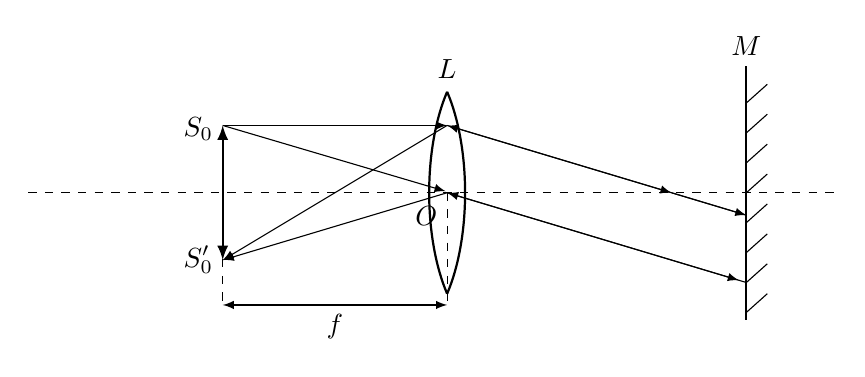
\begin{tikzpicture}[x=0.95cm,y=0.95cm,>=latex]
% principal axis
\draw[dashed] (-0.6,0) -- (10.2,0);
% lens
\draw[thick] (5,-1.35) .. controls (5.32,-0.6) and (5.32,0.6) .. (5,1.35);
\draw[thick] (5,-1.35) .. controls (4.68,-0.6) and (4.68,0.6) .. (5,1.35);
\node[above] at (5,1.4) {$L$};
\node[below left] at (5,-0.05) {$O$};
% object S0
\draw[->,thick] (2,0) -- (2,0.9);
\node[left] at (2.0,0.85) {$S_0$};
% mirror
\draw[thick] (9,-1.7) -- (9,1.7);
\foreach \y in {-1.6,-1.2,...,1.6} \draw (9,\y) -- (9.28,\y+0.25);
\node[above] at (9,1.7) {$M$};
% outgoing rays
\draw[->] (2,0.9) -- (5,0.9);
\draw[->] (5,0.9) -- (8,0);
\draw[->] (8,0) -- (9,-0.3);
\draw[->] (2,0.9) -- (4.98,0.02);
\draw[->] (5,0) -- (8.9,-1.17);
% returning rays
\draw[->] (9,-0.3) -- (5,0.9);
\draw[->] (5,0.9) -- (2,-0.9);
\draw[->] (9,-1.2) -- (5,0);
\draw[->] (5,0) -- (2,-0.9);
% image
\draw[->,thick] (2,0) -- (2,-0.9);
\node[left] at (2,-0.9) {$S_0'$};
% focal length
\draw[<->] (2,-1.5) -- (5,-1.5) node[midway,below] {$f$};
\draw[dashed] (2,0) -- (2,-1.5);
\draw[dashed] (5,0) -- (5,-1.5);
\end{tikzpicture}
\end{figbox}

\textbf{3. Measurement of the focal length of a convex lens by the two-image method}

The two-image method is also called the conjugate method. According to the laws of image formation by a convex lens, if the distance $D$ between the object and the image screen is kept unchanged and $D>4f$, then when the convex lens is moved between the object and the screen two images can be formed, as shown in Fig.~8.01(b). $S_0$ is the object screen and $P$ the image screen; 1 denotes the object, 2 the small image and 3 the large image. When the lens is at position $x_1$ it forms an inverted, magnified real image; when the lens is at position $x_2$ it forms an inverted, reduced real image. Let the absolute value of the distance between these two positions be $d$, and let the distance between position $x_2$ and the image screen be $v_2$. From Fig.~8.01(b), for position $x_1$,
\[
u_1=D-d-v_2,\qquad v_1=d+v_2,
\]
and for position $x_2$,
\[
u_2=D-v_2.
\]
Using the lens imaging formula (1), one can show that the focal length of the lens is
\begin{equation}
f=\frac{D^2-d^2}{4D}. \tag{2}
\end{equation}
In formula (2) the experimental condition $D>4f$ must be satisfied.

\begin{figbox}{8.01(b)}
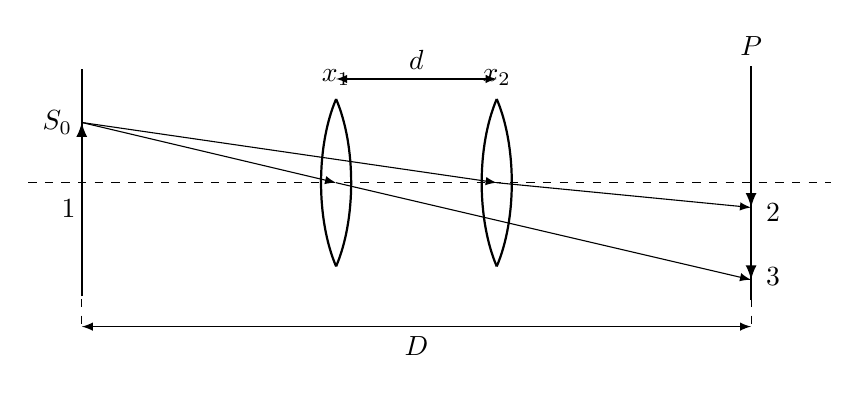
\begin{tikzpicture}[x=0.85cm,y=0.85cm,>=latex]
% axis
\draw[dashed] (-0.8,0) -- (11.2,0);
% object screen S0 with arrow
\draw[thick] (0,-1.7) -- (0,1.7);
\draw[->,thick] (0,0) -- (0,0.9);
\node[left] at (0,0.9) {$S_0$};
\node[below left] at (0.05,-0.1) {$1$};
% image screen P
\draw[thick] (10,-1.75) -- (10,1.75);
\node[above] at (10,1.75) {$P$};
% lenses
\foreach \x in {3.8,6.2}{
\draw[thick] (\x,-1.25) .. controls (\x+0.3,-0.55) and (\x+0.3,0.55) .. (\x,1.25);
\draw[thick] (\x,-1.25) .. controls (\x-0.3,-0.55) and (\x-0.3,0.55) .. (\x,1.25);
}
\node[above] at (3.8,1.3) {$x_1$};
\node[above] at (6.2,1.3) {$x_2$};
% rays through x1
\draw[->] (0,0.9) -- (3.8,0);
\draw[->] (3.8,0) -- (10,-1.45);
% rays through x2
\draw[->] (0,0.9) -- (6.2,0);
\draw[->] (6.2,0) -- (10,-0.37);
% images on screen
\draw[->,thick] (10,0) -- (10,-1.45);
\draw[->,thick] (10,0) -- (10,-0.37);
\node[right] at (10.08,-0.45) {$2$};
\node[right] at (10.08,-1.4) {$3$};
% D and d dimensions
\draw[<->] (0,-2.15) -- (10,-2.15) node[midway,below] {$D$};
\draw[dashed] (0,0) -- (0,-2.15);
\draw[dashed] (10,0) -- (10,-2.15);
\draw[<->] (3.8,1.55) -- (6.2,1.55) node[midway,above] {$d$};
\end{tikzpicture}
\end{figbox}

Usually, in measuring the focal length of a convex lens, the object, the lens holder and the screen are placed on an optical bench. However, the optical centre of the lens and the reading line on the lens holder base may not lie in the same plane, and hence a certain uncertainty exists. When the two-image method is used, $d=|x_2-x_1|$, which eliminates the systematic error introduced by the possible non-coplanarity of the optical centre of the lens and the reading line on the lens holder base. Of course, when the light source and the screen are not at the positions of the base reading lines, the value of the distance $D$ must still be corrected.

\subsection*{Experiment 8.02 \quad Measurement of the focal length of a concave lens by two different methods}

\textbf{[Apparatus and materials available]} Optical bench, convex lens, concave lens, object screen, image screen, plane mirror, etc.

\textbf{[Requirements]}

(1) Write down the principles and formulas of two different methods for measuring the focal length of a concave lens.

(2) Draw the experimental ray diagrams.

(3) Measure and calculate the focal length of the concave lens.

\textbf{Solution 8.02}\quad \textbf{1. Measurement of the focal length of a concave lens by the object-distance and image-distance method}

First use the convex lens $L_1$ to form a reduced, inverted real image $A'B'$ of the object $AB$, and then place the concave lens $L_2$ under test between the convex lens $L_1$ and the image $A'B'$, as shown in Fig.~8.02(a). If $O'A'<|f_{\mathrm{c}}|$ (where $f_{\mathrm{c}}$ is the focal length of the concave lens), then the beam that has passed through $L_1$, after refraction by $L_2$, still forms a real image $A''B''$. Note that for $L_2$ the image $A'B'$ is a virtual object and $A''B''$ is its real image, so that $u_2=-O'A'$ and $v_2=O'A''$. Substituting $u_2$ and $v_2$ into the lens focal-length formula
\[
\frac{1}{f}=\frac{1}{u}+\frac{1}{v},
\]
one can calculate the focal length $f_{\mathrm{c}}$ of the concave lens. The value of $f_{\mathrm{c}}$ is negative.

\begin{figbox}{8.02(a)}
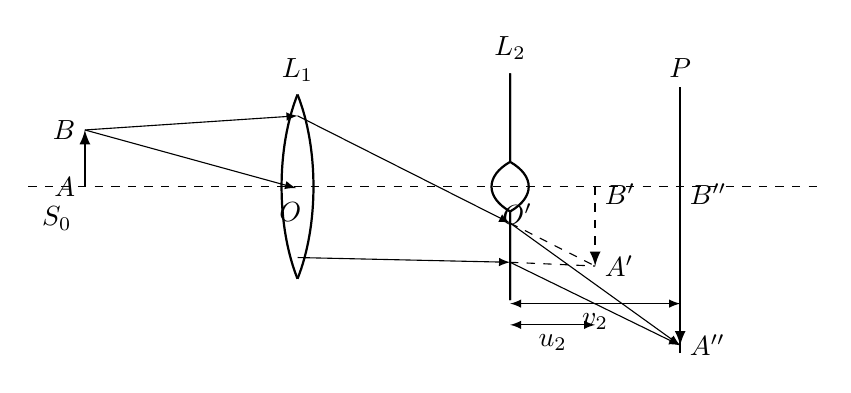
\begin{tikzpicture}[x=0.9cm,y=0.9cm,>=latex]
% axis
\draw[dashed] (-0.8,0) -- (10.4,0);
% object AB
\draw[->,thick] (0,0) -- (0,0.8);
\node[left] at (0,0.8) {$B$};
\node[left] at (0,0) {$A$};
\node[left] at (-0.05,-0.45) {$S_0$};
% L1 convex
\draw[thick] (3,-1.3) .. controls (3.3,-0.55) and (3.3,0.55) .. (3,1.3);
\draw[thick] (3,-1.3) .. controls (2.7,-0.55) and (2.7,0.55) .. (3,1.3);
\node[above] at (3,1.35) {$L_1$};
\node[below] at (2.9,-0.08) {$O$};
% L2 concave
\draw[thick] (6,-1.6) -- (6,-0.35) .. controls (5.65,-0.15) and (5.65,0.15) .. (6,0.35) -- (6,1.6);
\draw[thick] (6,-1.6) -- (6,-0.35) .. controls (6.35,-0.15) and (6.35,0.15) .. (6,0.35) -- (6,1.6);
\node[above] at (6,1.65) {$L_2$};
\node[below] at (6.1,-0.1) {$O'$};
% screen P
\draw[thick] (8.4,-2.35) -- (8.4,1.4);
\node[above] at (8.4,1.4) {$P$};
% rays from B through L1
\draw[->] (0,0.8) -- (3,1.0);
\draw[->] (3,1.0) -- (6,-0.514);
\draw[->] (6,-0.514) -- (8.4,-2.24);
\draw[->] (0,0.8) -- (2.98,-0.02);
\draw[->] (3,-1.0) -- (6,-1.067);
\draw[->] (6,-1.067) -- (8.4,-2.24);
% dashed continuation to virtual object A'
\draw[dashed] (6,-0.514) -- (7.2,-1.12);
\draw[dashed] (6,-1.067) -- (7.2,-1.12);
% virtual object A'B'
\draw[->,thick,dashed] (7.2,0) -- (7.2,-1.12);
\node[right] at (7.2,-1.12) {$A'$};
\node[right] at (7.2,-0.1) {$B'$};
% real image A''B''
\draw[->,thick] (8.4,0) -- (8.4,-2.24);
\node[right] at (8.4,-2.24) {$A''$};
\node[right] at (8.4,-0.1) {$B''$};
% dimensions u2 and v2
\draw[<->] (6,-1.95) -- (7.2,-1.95) node[midway,below] {$u_2$};
\draw[<->] (6,-1.65) -- (8.4,-1.65) node[midway,below] {$v_2$};
\end{tikzpicture}
\end{figbox}

In measuring the focal length of a concave lens, note the following. (1) Before the experiment, adjust the lenses so that the convex lens and the concave lens are coaxial and their principal axes are parallel to the scale of the optical bench. (2) Take care that the difference between the virtual object distance and the distance of the real image formed is not too small, so as to avoid too few significant figures. (3) Take care whether the optical centre of the lens and the screen lie on the reading line of the base; this can be checked by turning the lens through $180\degree$, and the error can be eliminated or reduced by readjusting for a sharp image.

\textbf{2. Measurement of the focal length of a concave lens by the autocollimation method}

A concave lens is a diverging lens. If a parallel beam is to be obtained with a concave lens, a convex lens must be used. First the convex lens $L_1$ forms an image of the point light source located at $S_0$ at $S_0'$. Record the reading of the position of $S_0'$ on the scale of the optical bench, as shown in Fig.~8.02(b). If the distance $OS_0'$ from the optical centre $O$ of $L_1$ to $S_0'$ satisfies $OS_0'>|f_{\mathrm{c}}|$, then place the concave lens $L_2$ under test and the plane mirror $M$ between $L_1$ and $S_0'$. When $L_2$ is moved so that the distance from the optical centre $O'$ of $L_2$ to $S_0'$ is $O'S_0'=|f|$, the beam emitted by the point source at $S_0$ becomes parallel after passing through $L_1$ and $L_2$, and after reflection by the plane mirror $M$ it forms a clear real image again at $S_0$. Once the positions of $S_0'$ and of $L_2$ (that is, $O'$) are determined, the focal length $f_{\mathrm{c}}$ of the concave lens can be measured.

\begin{figbox}{8.02(b)}
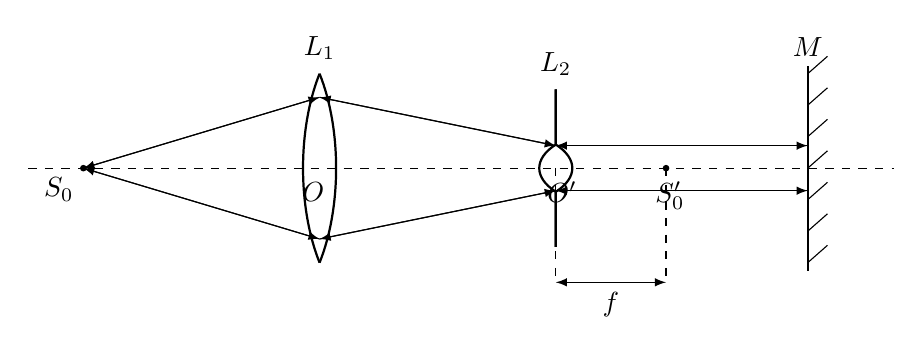
\begin{tikzpicture}[x=1.0cm,y=1.0cm,>=latex]
% axis
\draw[dashed] (-0.7,0) -- (10.3,0);
% S0 point source
\fill (0,0) circle (1.2pt);
\node[below left] at (0,0) {$S_0$};
% L1
\draw[thick] (3,-1.2) .. controls (3.28,-0.5) and (3.28,0.5) .. (3,1.2);
\draw[thick] (3,-1.2) .. controls (2.72,-0.5) and (2.72,0.5) .. (3,1.2);
\node[above] at (3,1.25) {$L_1$};
\node[below] at (2.92,-0.06) {$O$};
% L2 concave
\draw[thick] (6.0,-1.0) -- (6.0,-0.3) .. controls (5.72,-0.12) and (5.72,0.12) .. (6.0,0.3) -- (6.0,1.0);
\draw[thick] (6.0,-1.0) -- (6.0,-0.3) .. controls (6.28,-0.12) and (6.28,0.12) .. (6.0,0.3) -- (6.0,1.0);
\node[above] at (6,1.05) {$L_2$};
\node[below] at (6.08,-0.05) {$O'$};
% mirror
\draw[thick] (9.2,-1.3) -- (9.2,1.3);
\foreach \y in {-1.2,-0.8,...,1.2} \draw (9.2,\y) -- (9.45,\y+0.22);
\node[above] at (9.2,1.3) {$M$};
% focal point S0'
\fill (7.4,0) circle (1.2pt);
\node[below] at (7.45,-0.05) {$S_0'$};
% rays from S0 through L1 and L2: parallel after L2
\draw[->] (0,0) -- (3,0.9);
\draw[->] (3,0.9) -- (6,0.286);
\draw[->] (6,0.286) -- (9.2,0.286);
\draw[->] (0,0) -- (3,-0.9);
\draw[->] (3,-0.9) -- (6,-0.286);
\draw[->] (6,-0.286) -- (9.2,-0.286);
% reflected rays retrace their paths
\draw[->] (9.2,0.286) -- (6,0.286);
\draw[->] (6,0.286) -- (3,0.9);
\draw[->] (3,0.9) -- (0,0);
\draw[->] (9.2,-0.286) -- (6,-0.286);
\draw[->] (6,-0.286) -- (3,-0.9);
\draw[->] (3,-0.9) -- (0,0);
% f dimension
\draw[<->] (6,-1.45) -- (7.4,-1.45) node[midway,below] {$f$};
\draw[dashed] (6,0) -- (6,-1.45);
\draw[dashed] (7.4,0) -- (7.4,-1.45);
\end{tikzpicture}
\end{figbox}

\subsection*{Experiment 8.03 \quad Measurement of the focal length of a concave lens by the telescope method}

\textbf{[Apparatus and materials available]} Optical bench, light source, ground glass, convex lens, concave lens, Kepler telescope (to be adjusted by the experimenter), object and image screen, etc.

\textbf{[Requirements]}

(1) Draw the ray diagram.

(2) Write down the experimental method and the experimental steps.

(3) Obtain the experimental results.

\textbf{Solution 8.03}\quad \textbf{1.} The experimental ray diagram is shown in the figure. Since a telescope is usually used to observe distant objects, which produce approximately parallel light, the real image formed by the convex lens is a virtual object for the concave lens. If this virtual object of the concave lens is located at the focal point of the concave lens, the emergent light will be parallel. In this way the focal length $f_{\mathrm{c}}$ of the concave lens can be determined.

Method and steps:

(1) Adjust the light path so that the light source, the object, the convex lens, the concave lens, the telescope and so on are at the same height and coaxial, as shown in the figure.

(2) First use the convex lens to form an image of the object, and record the reading of the image position on the surface of the optical bench. Turn the lens round, form a clear image again, read the two readings and take their average.

(3) Direct the telescope at an object outside the window and make the image clear, that is, focus it at infinity; the parallax must be eliminated.

(4) Insert the concave lens under test between the convex lens and the telescope. Move the concave lens and change the distance until a clear image of the object is seen through the telescope; record the position of the concave lens. It must also be turned round; repeat this operation and read the scale. Take the average of the two readings.

(5) The difference between the position of the image formed by the convex lens and the reading of the position of the optical centre of the concave lens is then the focal length of the concave lens. Since the telescope forms an image only of parallel light, this shows that the object image lies in the focal plane of the concave lens.

The experimental data are omitted.

\begin{figbox}{8.03}
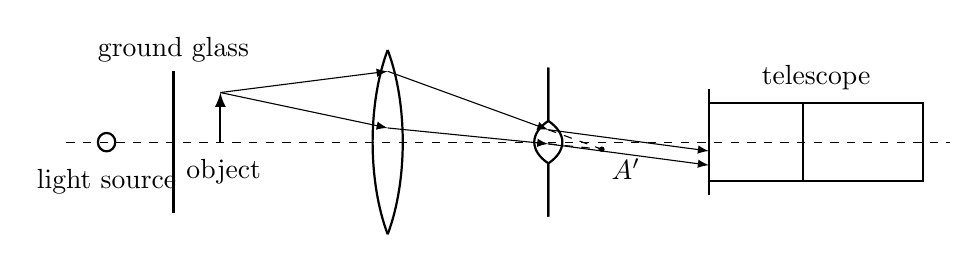
\begin{tikzpicture}[x=0.85cm,y=0.9cm,>=latex]
% bench line
\draw[dashed] (-0.6,0) -- (12.6,0);
% light source
\draw[thick] (0,0) circle (0.13);
\node[below] at (0,-0.25) {light source};
% ground glass
\draw[thick] (1.0,-1.0) -- (1.0,1.0);
\node[above] at (1.0,1.0) {ground glass};
% object arrow
\draw[->,thick] (1.7,0) -- (1.7,0.7);
\node[below] at (1.75,-0.1) {object};
% convex lens
\draw[thick] (4.2,-1.3) .. controls (4.5,-0.55) and (4.5,0.55) .. (4.2,1.3);
\draw[thick] (4.2,-1.3) .. controls (3.9,-0.55) and (3.9,0.55) .. (4.2,1.3);
% concave lens
\draw[thick] (6.6,-1.05) -- (6.6,-0.3) .. controls (6.32,-0.12) and (6.32,0.12) .. (6.6,0.3) -- (6.6,1.05);
\draw[thick] (6.6,-1.05) -- (6.6,-0.3) .. controls (6.88,-0.12) and (6.88,0.12) .. (6.6,0.3) -- (6.6,1.05);
% telescope
\draw[thick] (9.0,-0.55) rectangle (12.2,0.55);
\draw[thick] (9.0,-0.75) -- (9.0,0.75);
\draw[thick] (10.4,-0.55) -- (10.4,0.55);
\node[above] at (10.6,0.6) {telescope};
% rays from object tip through convex lens
\draw[->] (1.7,0.7) -- (4.2,1.0);
\draw[->] (4.2,1.0) -- (6.6,0.175);
\draw[->] (6.6,0.175) -- (9.0,-0.125);
\draw[->] (1.7,0.7) -- (4.2,0.2);
\draw[->] (4.2,0.2) -- (6.6,-0.025);
\draw[->] (6.6,-0.025) -- (9.0,-0.325);
% virtual image point A' (focal point of the concave lens)
\fill (7.4,-0.1) circle (1pt) node[below right] {$A'$};
\draw[dashed] (6.6,0.175) -- (7.4,-0.1);
\draw[dashed] (6.6,-0.025) -- (7.4,-0.1);
\end{tikzpicture}
\end{figbox}

\subsection*{Experiment 8.04 \quad Measurement of the focal length of the objective of the telescope and of the lens of the collimator on a spectrometer}

\textbf{[Apparatus and materials available]} Spectrometer, light source, plane reflecting mirror, ruler.

\textbf{[Requirements]}

(1) The optical axis of the telescope and the optical axis of the collimator on the spectrometer have already been adjusted perpendicular to the rotation axis of the instrument, and the two are coaxial; this adjustment is not to be made again.

(2) Draw the ray diagram of the measurement. For simplicity the object may be represented by a point object.

(3) Briefly describe the experimental procedure.

(4) Give the measurement results.

\textbf{Solution 8.04}\quad \textbf{1. Measurement of the focal length of the telescope objective}

(1) The experimental ray diagram is shown in Fig.~8.04(a).

(2) Procedure:

(i) Adjust the eyepiece so that the crosshairs are sharp, that is, the crosshairs lie in the focal plane of the eyepiece.

(ii) Adjust the objective and the platform so that the bright cross line forms a clear image, by reflection in the plane mirror, on the reticle on which the crosshairs lie. (The bright cross line is provided on the spectrometer telescope itself.)

(iii) Use a ruler to measure the distance from the telescope objective to the reticle several times and take the average value. This distance is the focal length $f_1$ of the telescope objective.

\begin{figbox}{8.04(a)}
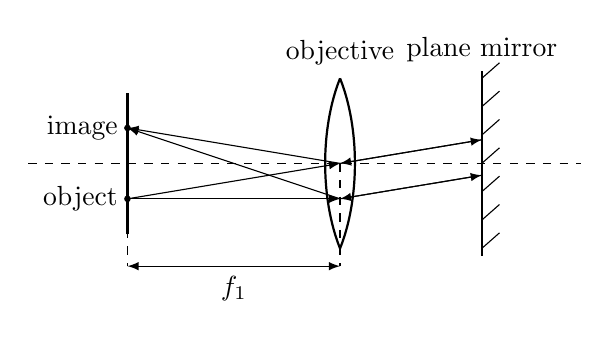
\begin{tikzpicture}[x=0.9cm,y=0.9cm,>=latex]
% axis
\draw[dashed] (1.6,0) -- (9.4,0);
% object/image plane
\draw[thick] (3,-1.0) -- (3,1.0);
\fill (3,-0.5) circle (1.2pt) node[left] {object};
\fill (3,0.5) circle (1.2pt) node[left] {image};
% objective lens
\draw[thick] (6,-1.2) .. controls (6.28,-0.5) and (6.28,0.5) .. (6,1.2);
\draw[thick] (6,-1.2) .. controls (5.72,-0.5) and (5.72,0.5) .. (6,1.2);
\node[above] at (6,1.25) {objective};
% plane mirror
\draw[thick] (8,-1.3) -- (8,1.3);
\foreach \y in {-1.2,-0.8,...,1.2} \draw (8,\y) -- (8.25,\y+0.22);
\node[above] at (8,1.3) {plane mirror};
% outgoing rays
\draw[->] (3,-0.5) -- (6,0);
\draw[->] (6,0) -- (8,0.333);
\draw[->] (3,-0.5) -- (6,-0.5);
\draw[->] (6,-0.5) -- (8,-0.167);
% returning rays
\draw[->] (8,0.333) -- (6,0);
\draw[->] (6,0) -- (3,0.5);
\draw[->] (8,-0.167) -- (6,-0.5);
\draw[->] (6,-0.5) -- (3,0.5);
% f dimension
\draw[<->] (3,-1.45) -- (6,-1.45) node[midway,below] {$f_1$};
\draw[dashed] (3,0) -- (3,-1.45);
\draw[dashed] (6,0) -- (6,-1.45);
\end{tikzpicture}
\end{figbox}

\textbf{2. Measurement of the focal length of the collimator lens}

(1) The ray diagram of the formation of the slit image on the reticle of the telescope is shown in Fig.~8.04(b). The telescope has previously been focused at infinity.

(2) Procedure:

Adjust the distance between the slit of the collimator and the lens so that the image of the slit observed through the telescope is sharpest. At this time the slit lies in the focal plane of the collimator. Use a ruler to measure the distance from the slit to the collimator lens several times and take the average value; this value is the focal length $f_2$ of the collimator lens.

\begin{figbox}{8.04(b)}
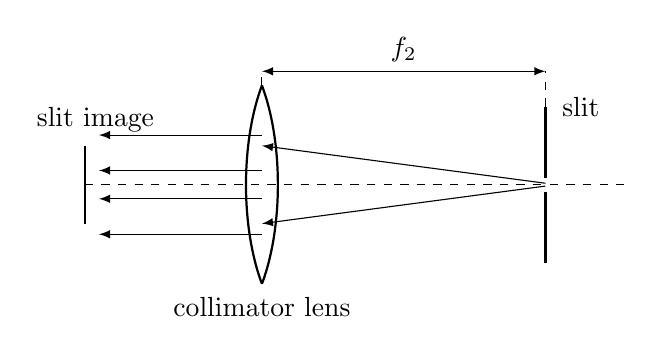
\begin{tikzpicture}[x=0.9cm,y=0.9cm,>=latex]
% optical axis
\draw[dashed] (-0.5,0) -- (7.2,0);
% collimator lens
\draw[thick] (2,-1.4) .. controls (2.3,-0.6) and (2.3,0.6) .. (2,1.4);
\draw[thick] (2,-1.4) .. controls (1.7,-0.6) and (1.7,0.6) .. (2,1.4);
\node[below] at (2,-1.45) {collimator lens};
% slit
\draw[thick] (6,-1.1) -- (6,-0.1);
\draw[thick] (6,0.1) -- (6,1.1);
\node[right] at (6.1,1.1) {slit};
% parallel beam to the left
\draw[->] (2,0.7) -- (-0.3,0.7);
\draw[->] (2,-0.7) -- (-0.3,-0.7);
\draw[->] (2,0.2) -- (-0.3,0.2);
\draw[->] (2,-0.2) -- (-0.3,-0.2);
% rays from slit to lens
\draw[->] (6,0.02) -- (2,0.55);
\draw[->] (6,-0.02) -- (2,-0.55);
% slit image
\draw[thick] (-0.5,-0.55) -- (-0.5,0.55);
\node[above] at (-0.35,0.6) {slit image};
% f2 dimension
\draw[<->] (2,1.6) -- (6,1.6) node[midway,above] {$f_2$};
\draw[dashed] (2,1.4) -- (2,1.6);
\draw[dashed] (6,1.1) -- (6,1.6);
\end{tikzpicture}
\end{figbox}

\subsection*{Experiment 8.05 \quad Measurement of the focal length of a concave mirror, and of the radii of curvature of a convex mirror and a concave mirror}

\textbf{[Apparatus and materials available]} Optical bench, screen with a ``1''-shaped aperture, arrow (pin), convex lens, convex mirror, concave mirror, lamp, etc.

\textbf{[Requirements]}

(1) Measure the focal length of the concave mirror, draw the ray diagram and write down the measurement formula.

(2) Measure the radius of curvature of the concave mirror, draw the ray diagram and write down the measurement formula.

(3) Measure the radius of curvature of the convex mirror.

\textbf{Solution 8.05}\quad \textbf{1. Measurement of the focal length of a concave mirror by the object-distance and image-distance method}

The experimental light path is shown in Fig.~8.05(a). The light source is an incandescent lamp. The object screen is a white screen with a hollow ``1''-shaped arrow cut in it; the arrow is above the optical axis. Another white half-screen is placed below the optical axis. With the object distance $S$ fixed, the white half-screen is moved until an inverted real image can be observed; the distance from the white half-screen to the spherical mirror is then the image distance $S'$. Using the spherical mirror imaging formula
\[
\frac{1}{S}+\frac{1}{S'}=\frac{1}{f},
\]
the focal length $f$ of the concave mirror can be obtained.

\begin{figbox}{8.05(a)}
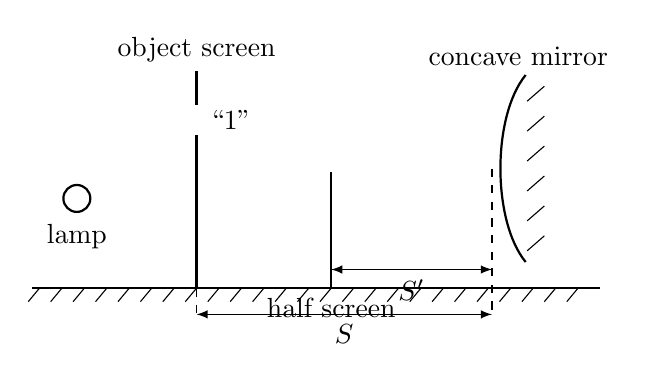
\begin{tikzpicture}[x=0.95cm,y=0.95cm,>=latex]
% bench
\draw[thick] (0,-1.6) -- (7.6,-1.6);
\foreach \x in {0.1,0.4,...,7.5} \draw (\x,-1.6) -- (\x-0.15,-1.78);
% lamp
\draw[thick] (0.6,-0.4) circle (0.18);
\node[below] at (0.6,-0.62) {lamp};
% object screen with 1-shaped aperture above axis
\draw[thick] (2.2,-1.6) -- (2.2,0.45);
\draw[thick] (2.2,0.85) -- (2.2,1.3);
\node[above] at (2.2,1.3) {object screen};
\node[right] at (2.25,0.65) {``1''};
% half screen below axis
\draw[thick] (4.0,-1.6) -- (4.0,-0.05);
\node[below] at (4.0,-1.6) {half screen};
% concave mirror
\draw[thick] (6.6,-1.25) .. controls (6.15,-0.7) and (6.15,0.7) .. (6.6,1.25);
\foreach \y in {-1.1,-0.7,...,1.1} \draw (6.62,\y) -- (6.85,\y+0.2);
\node[above] at (6.5,1.25) {concave mirror};
% dimensions
\draw[<->] (2.2,-1.95) -- (6.15,-1.95) node[midway,below] {$S$};
\draw[dashed] (2.2,-1.6) -- (2.2,-1.95);
\draw[dashed] (6.15,0) -- (6.15,-1.95);
\draw[<->] (4.0,-1.35) -- (6.15,-1.35) node[midway,below] {$S'$};
\end{tikzpicture}
\end{figbox}

\textbf{2. Measurement of the radius of curvature of a concave mirror by the parallax method}

A pin and the spherical mirror under test are placed perpendicular to the optical bench, as shown in Fig.~8.05(b). A small electric bulb illuminates the pin from the side. The observer looks along the surface of the optical bench (the inclined scale surface of the bench) at the object and at the real image formed by reflection in the concave mirror. When the concave mirror is moved and the observer sees the inverted real image formed by reflection in the mirror coincide with the original object, the distance between the pin and the concave mirror can be read from the scale on the bench; this is the radius of curvature of the concave mirror.

\begin{figbox}{8.05(b)}
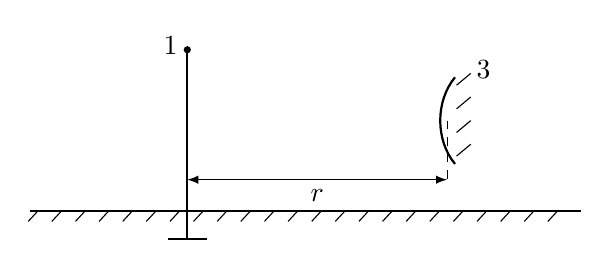
\begin{tikzpicture}[x=1.0cm,y=1.0cm,>=latex]
% bench (inclined scale surface)
\draw[thick] (0,-1.15) -- (7.0,-1.15);
\foreach \x in {0.1,0.4,...,6.9} \draw (\x,-1.15) -- (\x-0.12,-1.28);
% pin
\draw[thick] (2.0,-1.15) -- (2.0,0.9);
\fill (2.0,0.9) circle (1.3pt);
\node[left] at (2.0,0.95) {$1$};
% holder
\draw[thick] (2.0,-1.15) -- (2.0,-1.5);
\draw[thick] (1.75,-1.5) -- (2.25,-1.5);
% concave mirror
\draw[thick] (5.4,-0.55) .. controls (5.15,-0.25) and (5.15,0.25) .. (5.4,0.55);
\foreach \y in {-0.45,-0.15,0.15,0.45} \draw (5.42,\y) -- (5.6,\y+0.15);
\node[right] at (5.55,0.65) {$3$};
% dimension r
\draw[<->] (2.0,-0.75) -- (5.3,-0.75) node[midway,below] {$r$};
\draw[dashed] (2.0,0.9) -- (2.0,-0.75);
\draw[dashed] (5.3,0) -- (5.3,-0.75);
\end{tikzpicture}
\end{figbox}

\textbf{3. Determination of the radius of curvature of a convex mirror}

A convex mirror diverges a light beam, so the parallax method described above is not applicable to a convex mirror. A converging beam must be used to illuminate the convex mirror. The light path formed by the light source (object screen), the convex lens and the convex mirror is shown in Fig.~8.05(c). Move the convex mirror so that the centre of curvature of the convex mirror lies exactly at the convergence point of the original converging beam; then the converging beam, after reflection by the convex mirror, returns along its original path and forms a real image at the position of the object screen. Then move the convex mirror so that the centre of the mirror surface is exactly at the convergence point of the converging beam; then the light, after reflection by the convex mirror, still forms an image at the position of the original object screen. In this way the distance $r'$ through which the convex mirror is moved, taken with a negative sign, is the radius of curvature of the convex mirror:
\[
r=-r'.
\]

\begin{figbox}{8.05(c)}
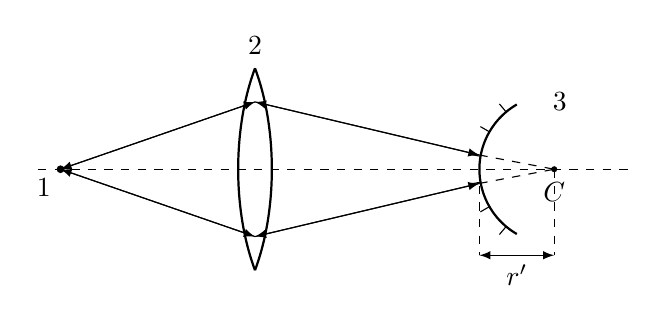
\begin{tikzpicture}[x=0.95cm,y=0.95cm,>=latex]
% axis
\draw[dashed] (0.3,0) -- (8.2,0);
% object point
\fill (0.6,0) circle (1.4pt) node[below left] {$1$};
% convex lens
\draw[thick] (3.2,-1.35) .. controls (3.5,-0.55) and (3.5,0.55) .. (3.2,1.35);
\draw[thick] (3.2,-1.35) .. controls (2.9,-0.55) and (2.9,0.55) .. (3.2,1.35);
\node[above] at (3.2,1.4) {$2$};
% convex mirror (vertex at 6.2, centre of curvature at 7.2)
\draw[thick] (6.7,-0.866) arc[start angle=240, end angle=120, radius=1.0];
\foreach \a in {130,150,170,190,210,230} \draw (7.2,0) ++(\a:1.0) -- ++(\a:0.14);
\node[right] at (7.05,0.9) {$3$};
% convergence point / centre of curvature
\fill (7.2,0) circle (1.1pt);
\node[below] at (7.2,-0.05) {$C$};
% rays
\draw[->] (0.6,0) -- (3.2,0.9);
\draw[->] (3.2,0.9) -- (6.2,0.19);
\draw[dashed] (6.2,0.19) -- (7.2,0);
\draw[->] (0.6,0) -- (3.2,-0.9);
\draw[->] (3.2,-0.9) -- (6.2,-0.19);
\draw[dashed] (6.2,-0.19) -- (7.2,0);
% reflected rays retrace
\draw[->] (6.2,0.19) -- (3.2,0.9);
\draw[->] (3.2,0.9) -- (0.6,0);
\draw[->] (6.2,-0.19) -- (3.2,-0.9);
\draw[->] (3.2,-0.9) -- (0.6,0);
% r' dimension
\draw[<->] (6.2,-1.15) -- (7.2,-1.15) node[midway,below] {$r'$};
\draw[dashed] (6.2,0) -- (6.2,-1.15);
\draw[dashed] (7.2,0) -- (7.2,-1.15);
\end{tikzpicture}
\end{figbox}

\subsection*{Experiment 8.06 \quad Measurement of the focal length of a convex lens group}

\textbf{[Apparatus and materials available]} One convex lens, one convex lens group, millimetre ruler, object screen, image screen, light source.

\textbf{[Requirement]} Use the magnification formula $V=f/x$ to measure the focal length $f$ of the convex lens group, where $V$ is the transverse magnification of the convex lens group, $x$ is the distance from the object to the object-side focal point of the convex lens group, and $f$ is the focal length of the convex lens group.

(1) Write down the measurement method and the steps.

(2) Draw a schematic diagram of the positions of the experimental measuring instruments.

(3) Record the original data; measure three times.

\textbf{Solution 8.06}\quad \textbf{1. Principle and steps of the measurement}

First the focal length of the single lens $L$ is measured by the displacement method. Then the distance from the single lens to the object screen is made equal to the focal length of the lens, the lens group under test is placed behind it, and the imaging position, that is, the position of the image-side focal point, is found with the image screen. The single lens is removed, the imaging position is found again, the sizes of the image and of the object are measured, and the transverse magnification $V$ is obtained. The difference between the two imaging positions is $x'$; substituting this into the measurement formula, the focal length $f$ can be calculated.

The measurement formula is $V=f/x$, where $V$ is the transverse magnification of the convex lens group, $x$ is the distance from the object to the object-side focal point of the lens group, and
\[
f=Vx=\frac{y'}{y}x',
\]
where $y'$ is the size of the image, $y$ the size of the object, $V=y'/y$, and $x'$ is the difference between the two imaging positions; it is more convenient to measure $x'$.

\textbf{2. Diagram of the measuring light path and arrangement}

\begin{figbox}{8.06(a)}
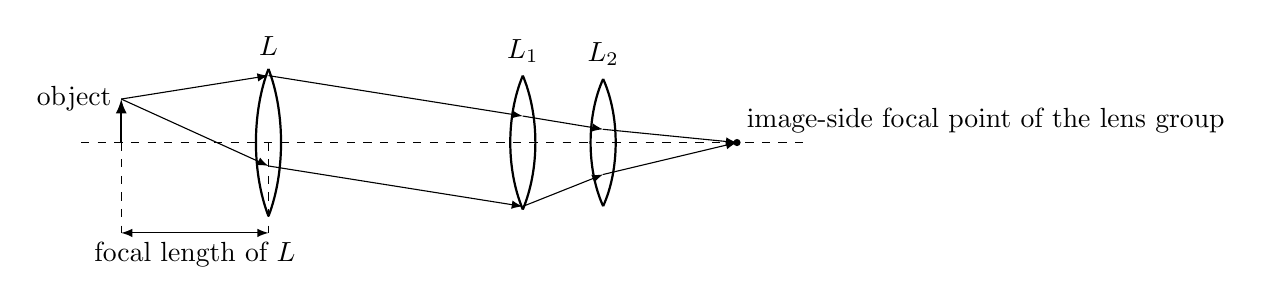
\begin{tikzpicture}[x=0.85cm,y=0.85cm,>=latex]
% axis
\draw[dashed] (-0.6,0) -- (10.2,0);
% object
\draw[->,thick] (0,0) -- (0,0.65);
\node[left] at (0,0.65) {object};
% single lens L
\draw[thick] (2.2,-1.1) .. controls (2.45,-0.45) and (2.45,0.45) .. (2.2,1.1);
\draw[thick] (2.2,-1.1) .. controls (1.95,-0.45) and (1.95,0.45) .. (2.2,1.1);
\node[above] at (2.2,1.15) {$L$};
% lens group
\draw[thick] (6.0,-1.0) .. controls (6.25,-0.4) and (6.25,0.4) .. (6.0,1.0);
\draw[thick] (6.0,-1.0) .. controls (5.75,-0.4) and (5.75,0.4) .. (6.0,1.0);
\node[above] at (6.0,1.05) {$L_1$};
\draw[thick] (7.2,-0.95) .. controls (7.45,-0.4) and (7.45,0.4) .. (7.2,0.95);
\draw[thick] (7.2,-0.95) .. controls (6.95,-0.4) and (6.95,0.4) .. (7.2,0.95);
\node[above] at (7.2,1.0) {$L_2$};
% rays from object tip: parallel bundle after L
\draw[->] (0,0.65) -- (2.2,1.0);
\draw[->] (2.2,1.0) -- (6.0,0.396);
\draw[->] (6.0,0.396) -- (7.2,0.198);
\draw[->] (7.2,0.198) -- (9.2,0);
\draw[->] (0,0.65) -- (2.2,-0.35);
\draw[->] (2.2,-0.35) -- (6.0,-0.954);
\draw[->] (6.0,-0.954) -- (7.2,-0.477);
\draw[->] (7.2,-0.477) -- (9.2,0);
% image-side focal point of the group
\fill (9.2,0) circle (1.3pt);
\node[above right] at (9.2,0) {image-side focal point of the lens group};
% focal length of L
\draw[<->] (0,-1.35) -- (2.2,-1.35) node[midway,below] {focal length of $L$};
\draw[dashed] (0,0) -- (0,-1.35);
\draw[dashed] (2.2,0) -- (2.2,-1.35);
\end{tikzpicture}
\end{figbox}

\begin{figbox}{8.06(b)}
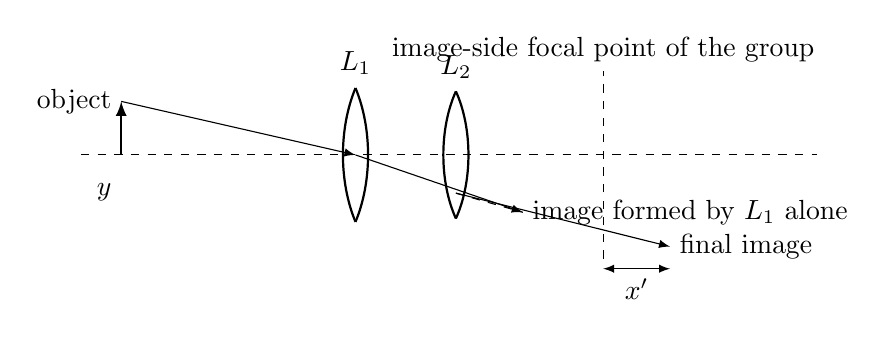
\begin{tikzpicture}[x=0.85cm,y=0.85cm,>=latex]
% axis
\draw[dashed] (-0.6,0) -- (10.4,0);
% object
\draw[->,thick] (0,0) -- (0,0.8);
\node[left] at (0,0.8) {object};
\node[left] at (0,-0.55) {$y$};
% lens group
\draw[thick] (3.5,-1.0) .. controls (3.75,-0.4) and (3.75,0.4) .. (3.5,1.0);
\draw[thick] (3.5,-1.0) .. controls (3.25,-0.4) and (3.25,0.4) .. (3.5,1.0);
\node[above] at (3.5,1.05) {$L_1$};
\draw[thick] (5.0,-0.95) .. controls (5.25,-0.4) and (5.25,0.4) .. (5.0,0.95);
\draw[thick] (5.0,-0.95) .. controls (4.75,-0.4) and (4.75,0.4) .. (5.0,0.95);
\node[above] at (5.0,1.0) {$L_2$};
% ray through L1 and its virtual image
\draw[->] (0,0.8) -- (3.5,0);
\draw[->] (3.5,0) -- (6.0,-0.857);
\draw[dashed] (5.0,-0.571) -- (6.0,-0.857);
\node[right] at (6.0,-0.857) {image formed by $L_1$ alone};
% ray after L2
\draw[->] (5.0,-0.571) -- (8.2,-1.37);
\node[right] at (8.2,-1.37) {final image};
% reference plane for the image-side focal point
\draw[dashed] (7.2,-1.55) -- (7.2,1.25);
\node[above] at (7.2,1.25) {image-side focal point of the group};
% x' dimension
\draw[<->] (7.2,-1.7) -- (8.2,-1.7) node[midway,below] {$x'$};
\end{tikzpicture}
\end{figbox}

\textbf{3. Example of experimental data}

\begin{center}
\textbf{Table 8.06-1}\quad Two-image method for measuring the focal length of the convex lens\\[3pt]
\begin{tabular}{cccc}
\toprule
Number & Object--screen distance $D/\mathrm{cm}$ & Displacement $d/\mathrm{cm}$ & Focal length$/\mathrm{cm}$ \\
\midrule
1 & 52.36 & 23.29 & 10.51 \\
2 & 52.35 & 23.56 & 10.48 \\
3 & 52.36 & 22.88 & 10.59 \\
\midrule
Average & 52.36 & 23.24 & 10.52 \\
\bottomrule
\end{tabular}
\end{center}

\begin{center}
\textbf{Table 8.06-2}\quad Measurement of the focal length of the lens group\\[3pt]
\begin{tabular}{cccccc}
\toprule
Number & Object height $y/\mathrm{cm}$ & Image height $y'/\mathrm{cm}$ & Magnification $V$ & Displacement $x'/\mathrm{cm}$ & Focal length $f/\mathrm{cm}$ \\
\midrule
1 & 1.62 & 0.83 & 1.952 & 3.70 & 7.22 \\
2 & 1.63 & 0.80 & 2.038 & 3.68 & 7.50 \\
3 & 1.62 & 0.78 & 2.077 & 3.57 & 7.42 \\
\midrule
Average & 1.623 & 0.803 & 2.022 & 3.65 & 7.38 \\
\bottomrule
\end{tabular}
\end{center}

The result is a focal length $f=\SI{7.38}{cm}$ for the convex lens group.

\begin{commentary}
This problem uses the magnification formula to measure the focal length of a lens group, which is a fairly typical method in the measurement of the focal length of lens groups.
\end{commentary}

\subsection*{Experiment 8.07 \quad Measurement of the focal length of a convex lens}

\textbf{[Apparatus and materials available]} Optical bench (with a short scale only near the light source, and no scale on the rest), light source, object screen, image screen (with a graduated scale on it), convex lens under test.

\textbf{[Requirements]}

(1) Draw the ray diagram and briefly write down the principle of the measurement and the formula.

(2) Measure the focal length of the convex lens.

\textbf{Solution 8.07}\quad \textbf{1. Principle of the experiment}

Since the optical bench has graduations only on the section near the object screen, and the image screen has graduations, one can use only the readings of the large image and the small image on the image screen, together with the displacement of the lens read on a section of the guide rail of the bench, to calculate the focal length of the convex lens.

\begin{figbox}{8.07(a)}
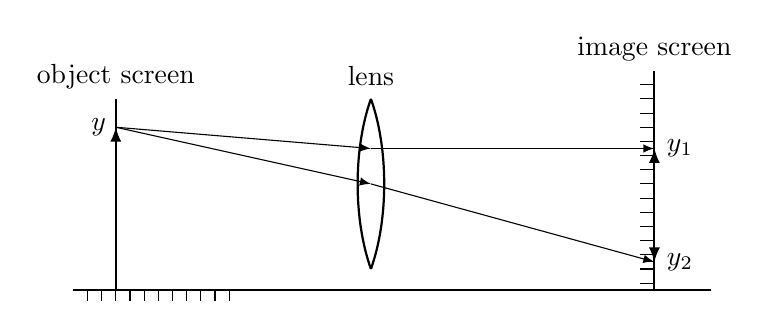
\begin{tikzpicture}[x=0.9cm,y=0.9cm,>=latex]
% bench
\draw[thick] (0,-1.5) -- (9.0,-1.5);
% short scale near the object
\foreach \x in {0.2,0.4,...,2.2} \draw (\x,-1.5) -- (\x,-1.65);
% object screen
\draw[thick] (0.6,-1.5) -- (0.6,1.2);
\draw[->,thick] (0.6,0) -- (0.6,0.8);
\node[left] at (0.6,0.8) {$y$};
\node[above] at (0.6,1.2) {object screen};
% lens
\draw[thick] (4.2,-1.2) .. controls (4.45,-0.5) and (4.45,0.5) .. (4.2,1.2);
\draw[thick] (4.2,-1.2) .. controls (3.95,-0.5) and (3.95,0.5) .. (4.2,1.2);
\node[above] at (4.2,1.25) {lens};
% image screen with scale
\draw[thick] (8.2,-1.5) -- (8.2,1.6);
\foreach \y in {-1.4,-1.2,...,1.5} \draw (8.2,\y) -- (8.0,\y);
\node[above] at (8.2,1.6) {image screen};
% images
\draw[->,thick] (8.2,0) -- (8.2,0.5);
\node[right] at (8.24,0.5) {$y_1$};
\draw[->,thick] (8.2,0) -- (8.2,-1.1);
\node[right] at (8.24,-1.1) {$y_2$};
% rays forming the images
\draw[->] (0.6,0.8) -- (4.2,0);
\draw[->] (4.2,0) -- (8.2,-1.1);
\draw[->] (0.6,0.8) -- (4.2,0.5);
\draw[->] (4.2,0.5) -- (8.2,0.5);
\end{tikzpicture}
\end{figbox}

\textbf{2. Experimental method}

(1) Find the object height $y$ by the conjugate method:
\begin{equation}
y=\sqrt{y_1y_2}, \tag{1}
\end{equation}
where $y_1$ and $y_2$ are the image heights in the two conjugate imagings.

(2) The first imaging is shown in Fig.~8.07(b)(1); we have
\[
\triangle OCF\sim\triangle A'B'F,
\]
so
\begin{equation}
\frac{x}{f}=\frac{A'B'}{AB}=\frac{A'B'}{y}, \tag{1}
\end{equation}
where $x$ is the length $FA'$.

\begin{figbox}{8.07(b)}
\begin{tikzpicture}[x=0.85cm,y=0.85cm,>=latex]
% ---------- panel (1) ----------
\begin{scope}[yshift=3.2cm]
\draw[dashed] (-0.5,0) -- (8.2,0);
% lens
\draw[thick] (4,-1.1) -- (4,1.1);
\draw (4,1.1) -- (3.85,0.9); \draw (4,1.1) -- (4.15,0.9);
\draw (4,-1.1) -- (3.85,-0.9); \draw (4,-1.1) -- (4.15,-0.9);
\node[below] at (4,-1.15) {$O$};
% object
\draw[thick] (0,0) -- (0,0.8);
\node[left] at (0,0.8) {$B$};
\node[left] at (0,0) {$A$};
% ray B -> O -> B'
\draw[->] (0,0.8) -- (3.98,0.01);
\draw[->] (4,0) -- (8,-0.8);
% horizontal from B to lens at C, then through F to B'
\draw (0,0.8) -- (4,0.8);
\draw[->] (4,0.8) -- (8,-0.8);
\node[above] at (4,0.8) {$C$};
% image
\draw[thick] (8,0) -- (8,-0.8);
\node[right] at (8,-0.8) {$B'$};
\node[right] at (8,0) {$A'$};
% focal point
\fill (6,0) circle (1.2pt) node[above] {$F$};
% x dimension
\draw[<->] (6,-0.95) -- (8,-0.95) node[midway,below] {$x$};
\node at (3.0,1.5) {(1)};
\end{scope}
% ---------- panel (2) ----------
\begin{scope}[yshift=-3.4cm]
\draw[dashed] (-0.5,0) -- (9.0,0);
% lens
\draw[thick] (3.5,-1.15) -- (3.5,1.15);
\draw (3.5,1.15) -- (3.35,0.95); \draw (3.5,1.15) -- (3.65,0.95);
\draw (3.5,-1.15) -- (3.35,-0.95); \draw (3.5,-1.15) -- (3.65,-0.95);
\node[below] at (3.5,-1.2) {$O$};
% object
\draw[thick] (0,0) -- (0,0.8);
\node[left] at (0,0.8) {$B$};
\node[left] at (0,0) {$A$};
% ray B -> O -> B''
\draw[->] (0,0.8) -- (3.48,0.01);
\draw[->] (3.5,0) -- (8.2,-1.07);
% horizontal from B to lens at C, then through F to B''
\draw (0,0.8) -- (3.5,0.8);
\draw[->] (3.5,0.8) -- (8.2,-1.07);
\node[above] at (3.5,0.8) {$C$};
% image
\draw[thick] (8.2,0) -- (8.2,-1.07);
\node[right] at (8.2,-1.07) {$B''$};
\node[right] at (8.2,0) {$A''$};
% focal point
\fill (5.5,0) circle (1.2pt) node[above] {$F$};
% x+b dimension
\draw[<->] (5.5,-1.25) -- (8.2,-1.25) node[midway,below] {$x+b$};
\node at (2.6,1.5) {(2)};
\end{scope}
\end{tikzpicture}
\end{figbox}

(3) The second imaging is shown in Fig.~8.07(b)(2); we have $\triangle OCF\sim\triangle A''B''F$, so
\begin{equation}
\frac{x+b}{f}=\frac{A''B''}{AB}=\frac{A''B''}{y}, \tag{2}
\end{equation}
where $b$ is the displacement of the convex lens in the two imagings.

From (1) and (2),
\[
\frac{A'B'}{y}-\frac{A''B''}{y}=\frac{x}{f}-\frac{x+b}{f},
\]
so
\[
f=\frac{by}{A''B''-A'B'}.
\]

\begin{commentary}
A lens is a basic element of all kinds of optical instruments. Mastering the laws of lens imaging and learning to analyse and adjust light paths is useful for understanding the construction and the correct use of optical instruments. The focal length is an important characteristic parameter of a lens; lenses of suitable focal length must be chosen on different occasions, so the measurement of the focal length of a lens is very important.
\end{commentary}

\subsection*{Experiment 8.08 \quad Measurement of the focal length $f$ and the radius of curvature $R$ of a thin symmetric biconcave lens, and calculation of the refractive index $n$ from them}

\textbf{[Apparatus and materials available]} Optical bench, light source, pinhole object screen, image screen, thin convex lens, thin symmetric biconcave lens under test whose two surfaces have the same radius of curvature, one fine thread, white paper, adhesive tape, scissors, etc.

\textbf{[Requirements]}

(1) Briefly describe the measuring method and write down the measuring formula.

(2) Measure the focal length $f$ of the thin biconcave lens.

(3) Measure the radius of curvature $R$ of the thin biconcave lens.

(4) From the focal length $f$ and the radius of curvature $R$ of the thin biconcave lens, find the value of the refractive index $n$.

\textbf{Solution 8.08}\quad \textbf{1.} In this experiment the two-image method is first used to measure the focal length $f_1$ of the convex lens; the ray diagram is as shown in Fig.~8.01(b). Then the concave lens is placed between the convex lens and the image. The image of the convex lens is a virtual object for the concave lens; the focal length $f_2$ of the concave lens is measured by the object-distance and image-distance method. The radii of curvature $R_1$ and $R_2$ of the biconcave lens can be measured by the method of Fig.~8.05(b). Applying the thin-lens focal-length formula
\[
\frac{1}{f}=(n-1)\left(\frac{1}{R_1}-\frac{1}{R_2}\right),
\]
we obtain
\[
n=1+\frac{1}{f\left(\dfrac{1}{R_1}-\dfrac{1}{R_2}\right)}.
\]

\textbf{2. Experimental results}

\begin{center}
\textbf{Table 8.08-1}\quad Measurement of the focal length of the convex lens\\[3pt]
\begin{tabular}{cccc}
\toprule
Number & Object--screen distance $D/\mathrm{cm}$ & Displacement $d/\mathrm{cm}$ & Focal length $f_1/\mathrm{cm}$ \\
\midrule
1 & 40.00 & 10.39 & \\
2 & 40.00 & 10.42 & \\
3 & 40.00 & 10.36 & \\
\midrule
Average & 40.00 & 10.39 & 9.33 \\
\bottomrule
\end{tabular}
\end{center}

\begin{center}
\textbf{Table 8.08-2}\quad Focal length of the concave lens\\[3pt]
\begin{tabular}{ccccccc}
\toprule
\multicolumn{3}{c}{Object distance$/\mathrm{cm}$} & \multicolumn{3}{c}{Image distance$/\mathrm{cm}$} & Focal length$/\mathrm{cm}$ \\
\cmidrule(lr){1-3}\cmidrule(lr){4-6}
$S_4$ & $S_3$ & $S_4-S_3$ & $S_5$ & $S_3$ & $S_5-S_3$ & $f$ \\
\midrule
42.50 & 35.00 & 7.50 & 47.40 & 35.00 & 12.40 & $-18.98$ \\
\bottomrule
\end{tabular}
\end{center}

\begin{center}
\textbf{Table 8.08-3}\quad Measurement of the radii of curvature of the concave lens (parallax method)\\[3pt]
\begin{tabular}{ccc}
\toprule
Position of the concave lens$/\mathrm{cm}$ & Position of the image of the left concave surface$/\mathrm{cm}$ & Position of the image of the right concave surface$/\mathrm{cm}$ \\
\midrule
5.00 & 27.76 & 28.89 \\
\bottomrule
\end{tabular}
\end{center}

\[
R_1=-(27.76-5.00)=-22.76\ (\mathrm{cm});\qquad R_2=28.89-5.00=23.89\ (\mathrm{cm}).
\]

Hence the refractive index of the glass is
\[
n=1+\frac{1}{f\left(\dfrac{1}{R_1}-\dfrac{1}{R_2}\right)}
=1+\frac{1}{(-18.98)\left(-\dfrac{1}{22.76}-\dfrac{1}{23.89}\right)}=1.614.
\]

The radius of curvature of a concave mirror is twice its focal length, $R=2f$. Therefore one may also use the collimator method or another method to measure the focal length of the concave mirror, and multiply it by 2 to obtain the radius of curvature.

\begin{commentary}
The method described in this problem can measure the refractive index of the material of a concave lens. With a different line of thought, if the refractive index of the glass is known, the focal length of a biconcave lens can also be measured by the above method.
\end{commentary}

\subsection*{Experiment 8.09 \quad Measurement of the refractive index of a liquid}

\textbf{[Apparatus and materials available]} Opaque square box, ruler, set square, liquid under test (in a beaker).

\textbf{[Requirements]}

(1) Draw the ray diagram and derive the measuring formula.

(2) Calculate the result.

\textbf{Solution 8.09}\quad \textbf{1.} The ray diagram is shown in Fig.~8.09(a).

Make a mark on the bottom edge of the square box (for example, put a coin there) and observe it with the eye along the upper edge of the box. When there is no water (liquid under test), the angle $\alpha$ is
\[
\sin\alpha=\frac{d}{\sqrt{h^2+d^2}},
\]
and when the liquid under test is present, the angle $\beta$ is
\[
\sin\beta=\frac{s}{\sqrt{s^2+l^2}}.
\]
By the refraction formula
\begin{equation}
n_{\text{water}}\sin\alpha=n_{\text{air}}\sin\beta. \tag{1}
\end{equation}
In formula (1), $\sin\alpha=\dfrac{d}{\sqrt{h^2+d^2}}$, $\sin\beta=\dfrac{s}{\sqrt{s^2+l^2}}$, and $n_{\text{air}}=1$, so the refractive index is
\begin{equation}
n_{\text{water}}=\frac{\sin\beta}{\sin\alpha}
=\frac{s}{\sqrt{s^2+l^2}}\cdot\frac{\sqrt{h^2+d^2}}{d}. \tag{2}
\end{equation}

\begin{figbox}{8.09(a)}
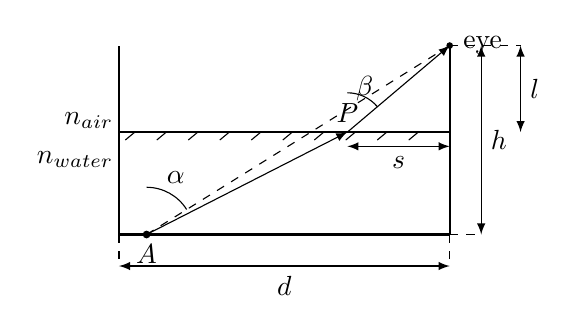
\begin{tikzpicture}[x=1.0cm,y=1.0cm,>=latex]
% box
\draw[thick] (0,0) -- (0,2.4) (0,0) -- (4.2,0) (4.2,0) -- (4.2,2.4);
% liquid
\draw[thick] (0,1.3) -- (4.2,1.3);
\foreach \x in {0.2,0.6,...,4.0} \draw (\x,1.3) -- (\x-0.12,1.2);
\node[left] at (0.05,1.45) {$n_{\text{air}}$};
\node[left] at (0.05,0.95) {$n_{\text{water}}$};
% mark A
\fill (0.35,0) circle (1.4pt) node[below] {$A$};
% eye at the upper edge
\fill (4.2,2.4) circle (1.2pt);
\node[right] at (4.25,2.4) {eye};
% ray without liquid (dashed)
\draw[dashed] (0.35,0) -- (4.2,2.4);
% ray with liquid
\draw[->] (0.35,0) -- (2.9,1.3);
\draw[->] (2.9,1.3) -- (4.2,2.4);
\node[above] at (2.9,1.3) {$P$};
% angles
\draw (0.35,0.6) arc (90:32:0.6);
\node at (0.72,0.72) {$\alpha$};
\draw (2.9,1.8) arc (90:40:0.5);
\node at (3.12,1.85) {$\beta$};
% dimensions
\draw[<->] (0,-0.4) -- (4.2,-0.4) node[midway,below] {$d$};
\draw[<->] (4.6,0) -- (4.6,2.4) node[midway,right] {$h$};
\draw[<->] (5.1,1.3) -- (5.1,2.4) node[midway,right] {$l$};
\draw[<->] (2.9,1.12) -- (4.2,1.12) node[midway,below] {$s$};
\draw[dashed] (4.2,0) -- (4.6,0);
\draw[dashed] (4.2,2.4) -- (5.1,2.4);
\draw[dashed] (0,0) -- (0,-0.4);
\draw[dashed] (4.2,0) -- (4.2,-0.4);
\end{tikzpicture}
\end{figbox}

\textbf{2.} The second method is as follows. Press a ruler tightly against the inner wall of the square box on the opposite side, and place the box at a certain position beside a support or the edge of a set square. Bring the eye close to the support or the set square and observe. When the box contains water, the eye observes the point $A$ at the bottom edge of the box, and the light path is the straight line $CBA$. Then pour all the water out of the box and observe with the eye from the original position $C$; the light path is the straight line $CBA'$.

From Fig.~8.09(b),
\begin{equation}
n_{\text{water}}=\frac{\sin i}{\sin\alpha}
=\frac{D/A'B}{D/AB}=\frac{AB}{A'B}
=\frac{\sqrt{D^2+h^2}}{\sqrt{D^2+(h-h')^2}}. \tag{3}
\end{equation}
In formula (3), $h'$ is the height $AA'$.

The experimental data are omitted.

\begin{figbox}{8.09(b)}
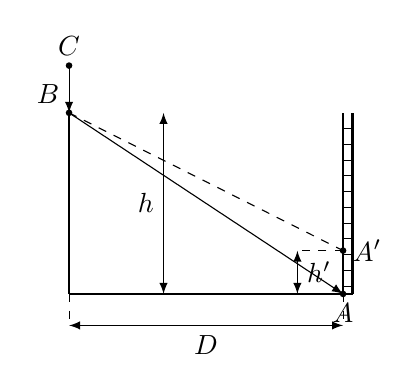
\begin{tikzpicture}[x=1.0cm,y=1.0cm,>=latex]
% box
\draw[thick] (0,0) -- (0,2.3) (0,0) -- (3.6,0) (3.6,0) -- (3.6,2.3);
% ruler against the far inner wall
\draw[thick] (3.48,0) -- (3.48,2.3);
\foreach \y in {0.1,0.3,...,2.2} \draw (3.48,\y) -- (3.58,\y);
% points A and A' on the far wall
\fill (3.48,0) circle (1.2pt) node[below] {$A$};
\fill (3.48,0.55) circle (1.2pt) node[right] {$A'$};
% point B at the top of the near wall
\fill (0,2.3) circle (1.2pt) node[above left] {$B$};
% eye at C
\fill (0,2.9) circle (1.2pt) node[above] {$C$};
% rays
\draw[->] (0,2.9) -- (0,2.3);
\draw[->] (0,2.3) -- (3.48,0);
\draw[dashed] (0,2.3) -- (3.48,0.55);
% D, h, h'
\draw[<->] (0,-0.4) -- (3.48,-0.4) node[midway,below] {$D$};
\draw[<->] (1.2,0) -- (1.2,2.3) node[midway,left] {$h$};
\draw[<->] (2.9,0) -- (2.9,0.55) node[midway,right] {$h'$};
\draw[dashed] (3.48,0) -- (2.9,0);
\draw[dashed] (3.48,0.55) -- (2.9,0.55);
\draw[dashed] (0,0) -- (0,-0.4);
\draw[dashed] (3.48,0) -- (3.48,-0.4);
\end{tikzpicture}
\end{figbox}

\subsection*{Experiment 8.10 \quad Determination of the refractive index of a craft glass ball}

\textbf{[Apparatus and materials available]} Optical bench, one small bulb ($12\,\mathrm{V}$), one power supply, object screen, image screen, stage, steel tape, vernier caliper, glass ball under test, ground glass, etc.

\textbf{[Requirements]}

(1) Write down the experimental method and derive the measuring formula.

(2) Briefly describe the experimental steps.

(3) Record the experimental data and calculate the result.

(4) Explain the main sources of experimental error.

\textbf{Solution 8.10}\quad \textbf{1. Experimental method and derivation of the measuring formula}

With the apparatus provided, the object can be made to form an image on the screen; the object distance, the image distance and the diameter of the ball are measured separately and substituted into the measuring formula. The experimental light path is as shown in the figure.

Let $SO=u$ and $OS'=v$.

By the law of refraction,
\begin{equation}
n=\frac{\sin i}{\sin\varphi}=\frac{\sin i'}{\sin\varphi'}. \tag{1}
\end{equation}
By the sine rule,
\[
\frac{u}{\sin i}=\frac{r}{\sin\alpha},\qquad
\frac{v}{\sin i'}=\frac{r}{\sin\beta}.
\]
By the geometrical relations,
\begin{equation}
\varphi+\varphi'=(i-\alpha)+(i'-\beta). \tag{2}
\end{equation}
Under paraxial conditions the angles $\alpha$, $\beta$, $i$, $i'$, $\varphi$, $\varphi'$ are all small, so
\begin{equation}
n=\frac{i}{\varphi},\qquad n=\frac{i'}{\varphi'},\qquad
\frac{i}{\alpha}=\frac{u}{r},\qquad \frac{i'}{\beta}=\frac{v}{r}. \tag{3}
\end{equation}
Substituting (3) into (2), we obtain
\begin{equation}
n=\frac{\alpha uv}{\alpha uv-r(u+v)}. \tag{4}
\end{equation}

\begin{figbox}{8.10}
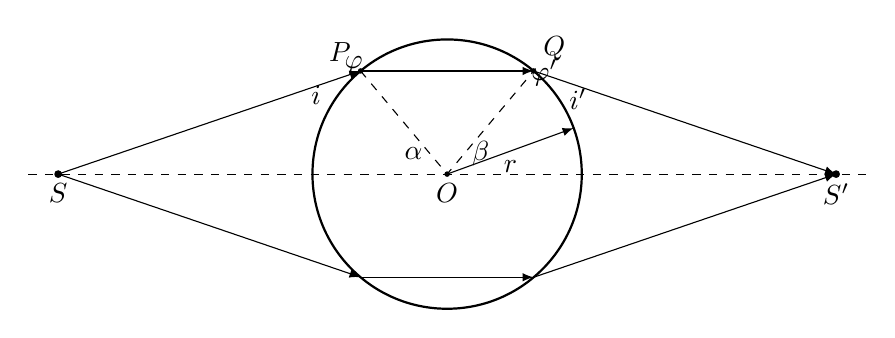
\begin{tikzpicture}[x=0.95cm,y=0.95cm,>=latex]
% glass ball
\draw[thick] (0,0) circle (1.8);
\fill (0,0) circle (1pt) node[below] {$O$};
% axis
\draw[dashed] (-5.6,0) -- (5.6,0);
% object and image
\fill (-5.2,0) circle (1.4pt) node[below] {$S$};
\fill (5.2,0) circle (1.4pt) node[below] {$S'$};
% entry and exit points
\coordinate (P) at (130:1.8);
\coordinate (Q) at (50:1.8);
\fill (P) circle (1pt) node[above left] {$P$};
\fill (Q) circle (1pt) node[above right] {$Q$};
% rays
\draw[->] (-5.2,0) -- (P);
\draw[->] (P) -- (Q);
\draw[->] (Q) -- (5.2,0);
\draw[->] (-5.2,0) -- (230:1.8);
\draw[->] (230:1.8) -- (310:1.8);
\draw[->] (310:1.8) -- (5.2,0);
% normals
\draw[dashed] (P) -- (0,0) -- (Q);
% radius
\draw[->] (0,0) -- (20:1.8) node[midway,below] {$r$};
% labels of angles
\node at (-1.75,1.05) {$i$};
\node at (-1.25,1.45) {$\varphi$};
\node at (1.3,1.35) {$\varphi'$};
\node at (1.75,1.0) {$i'$};
\node at (-0.45,0.28) {$\alpha$};
\node at (0.45,0.28) {$\beta$};
\end{tikzpicture}
\end{figbox}

\textbf{2. Experimental steps}

Adjust the apparatus on the optical bench so that the light source, the object screen, the craft glass ball and the image screen are at the same height and coaxial, and the light emitted by the object screen is imaged clearly on the image screen by the glass ball (lens). Measure the object distance and the image distance, and use a vernier caliper to measure the diameter $2r$ of the glass ball.

\textbf{3.} The experimental data are omitted. The main error of the experiment comes from the inaccurate determination of the image plane.

\subsection*{Experiment 8.11 \quad Measurement, with a spectrometer, of the angle of incidence on a prism and the angle of refraction of the emergent ray when the condition of minimum deviation is satisfied, and measurement of the minimum deviation angle}

\textbf{[Apparatus and materials available]} Spectrometer, prism, sodium lamp.

\textbf{[Requirements]}

(1) Measure the minimum deviation angle $\delta_0$ of the prism and the corresponding angles of incidence and emergence.

(2) Briefly explain the measuring method and draw a simple schematic diagram.

(3) Give the measurement results.

Note: the spectrometer has already been adjusted, so measurements can be made directly. On no account adjust the levelling screws of the telescope, of the collimator or of the stage, lest the measurement conditions be destroyed.

\textbf{Solution 8.11}\quad \textbf{1.} The angle of incidence is $55\degree30'0''$, the angle of refraction is $55\degree30'0''$, and the minimum deviation angle is $51\degree0'0''$.

\textbf{2.} The experimental light path is as shown in the figure.

\textbf{3. Minimum deviation angle:} place the prism on the stage, find the spectral line, and rotate the stage to change the angle of incidence while the telescope follows the emergent spectral line. If the line moves in the direction in which the deviation angle decreases, the stage is being rotated in the correct direction; when a certain position is reached, the spectral line no longer moves forward but begins to move in the opposite direction. This turning position is the position of minimum deviation. Measure its azimuth, then measure the azimuth of the incident light; subtracting the two gives the minimum deviation angle.

\textbf{4. Angle of incidence:} measure the azimuths of the incident light and of the normal to the corresponding face of the prism, and subtract them to obtain the angle between them; the supplement of this angle is the angle of incidence.

\textbf{Angle of refraction:} measure the azimuths of the emergent light from the prism and of the corresponding normal, and subtract them to obtain the angle between them, which is the angle of refraction.

\begin{figbox}{8.11}
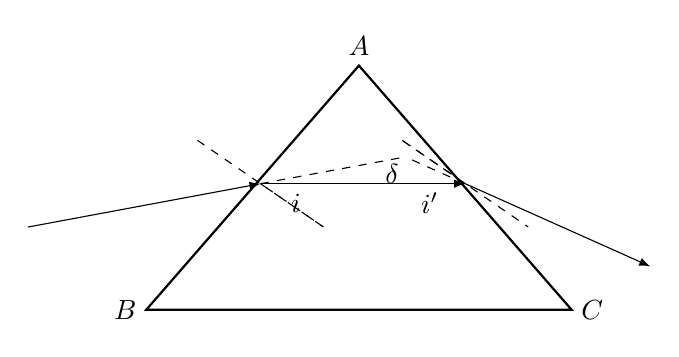
\begin{tikzpicture}[x=1.0cm,y=1.0cm,>=latex]
% prism
\coordinate (A) at (3,3.1);
\coordinate (B) at (0.3,0);
\coordinate (C) at (5.7,0);
\draw[thick] (A) -- (B) -- (C) -- cycle;
\node[above] at (A) {$A$};
\node[left] at (B) {$B$};
\node[right] at (C) {$C$};
% incident ray
\coordinate (P) at (1.75,1.6);
\draw[->] (-1.2,1.05) -- (P);
% inside
\coordinate (Q) at (4.35,1.6);
\draw[->] (P) -- (Q);
% emergent ray
\draw[->] (Q) -- (6.7,0.55);
% normals
\draw[dashed] (0.95,2.15) -- (2.55,1.05);
\draw[dashed] (3.55,2.15) -- (5.15,1.05);
\draw[dashed] (P) -- (2.55,1.05);
\draw[dashed] (Q) -- (3.55,2.15);
% deviation angle marked at the crossing of the extended rays
\draw[dashed] (P) -- (3.59,1.94);
\draw[dashed] (Q) -- (3.59,1.94);
\node at (3.42,1.72) {$\delta$};
\node at (2.2,1.35) {$i$};
\node at (3.9,1.35) {$i'$};
\end{tikzpicture}
\end{figbox}

\subsection*{Experiment 8.12 \quad Measurement of the refractive index of prism material}

\textbf{[Apparatus and materials available]} Prism, set square, white paper, etc.

\textbf{[Requirements]}

(1) The optical surfaces must not be measured in direct contact with paper, and the optical surfaces must not be touched with the hands.

(2) Draw the measuring ray diagram and write down the measuring formula.

(3) Measure and calculate the result.

\textbf{Solution 8.12}\quad \textbf{1.} The ray diagram is as shown in the figure.

\begin{figbox}{8.12}
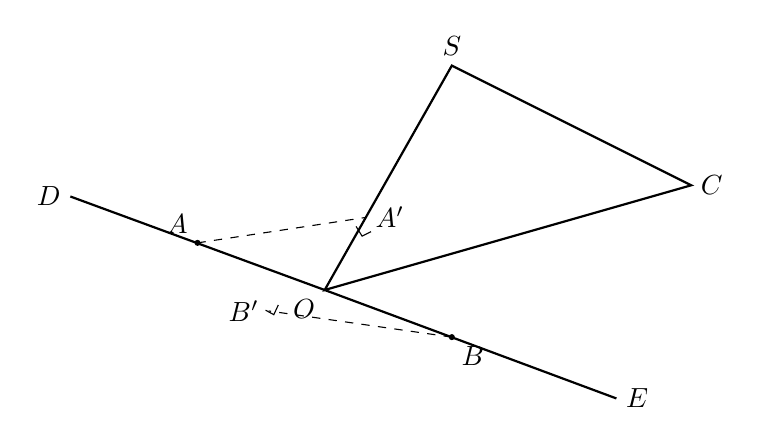
\begin{tikzpicture}[x=0.95cm,y=0.95cm,>=latex]
% prism
\coordinate (O) at (0,0);
\coordinate (S) at (1.7,3.0);
\coordinate (C) at (4.9,1.4);
\draw[thick] (O) -- (S) -- (C) -- cycle;
\node[below left] at (O) {$O$};
\node[above] at (S) {$S$};
\node[right] at (C) {$C$};
% line DE through O
\draw[thick] (-3.4,1.25) -- (O) -- (3.9,-1.45);
\node[left] at (-3.4,1.25) {$D$};
\node[right] at (3.9,-1.45) {$E$};
% points A and B with OA = OB
\fill (-1.7,0.63) circle (1.1pt) node[above left] {$A$};
\fill (1.7,-0.63) circle (1.1pt) node[below right] {$B$};
% perpendiculars
\coordinate (A1) at (0.55,0.97);
\coordinate (B1) at (-0.75,-0.28);
\draw[dashed] (-1.7,0.63) -- (A1);
\draw[dashed] (1.7,-0.63) -- (B1);
\node[right] at (A1) {$A'$};
\node[left] at (B1) {$B'$};
% right angle marks
\draw (0.42,0.85) -- (0.5,0.72) -- (0.62,0.78);
\draw (-0.62,-0.2) -- (-0.68,-0.33) -- (-0.79,-0.27);
\end{tikzpicture}
\end{figbox}

\textbf{2. Experimental method}

The vertex $O$ of the prism lies on the straight line $DE$. The prism is rotated about $O$ and observed from the direction of $D$ until the other vertex $S$ coincides with the straight line $DO$ (that is, lies on the same straight line). Take $OA=OB$; then the refractive index of the prism material is
\[
n=\frac{\sin r}{\sin i}=\frac{BB'}{AA'},
\]
where $BB'$ is the length of the perpendicular from $B$ to the straight line $OD$, and $AA'$ is the length of the perpendicular from $A$ to the straight line $OS$.

By the above graphical construction the refractive index $n$ of the prism material can be obtained. The experimental data are omitted.

\subsection*{Experiment 8.13 \quad Measurement of the refractive index of a prism (minimum deviation method)}

\textbf{[Apparatus and materials available]} Spectrometer, mercury lamp, prism.

\textbf{[Requirements]}

(1) Measure the minimum deviation angle $\delta_{\min}$ of the prism.

(2) Measure the apex angle of the prism.

(3) Calculate the refractive index of the prism for sodium light.

Note: the spectrometer has already been adjusted, so measurements can be made directly.

\textbf{Solution 8.13}\quad \textbf{1.} The experimental light path is as shown in Fig.~8.11.

\textbf{2.} The scale division of the spectrometer is $1'$, and the prism under test is No.~7.

The apex angle of the prism measured with the spectrometer is $A=60\degree1.8'$.

\textbf{3.} $\delta_{\min}$ is the minimum deviation angle. For an equilateral prism, $\delta_{\min}$ is the angle between the incident ray and the emergent ray when the angle of incidence is equal to the angle of emergence. The refractive index of the prism for sodium light is
\[
n=\frac{\sin\dfrac{\delta_{\min}+A}{2}}{\sin\dfrac{A}{2}},
\]
where $A$ is the apex angle of the prism.

The minimum deviation angle of the prism was measured for $\lambda=577.0\,\mathrm{nm}$ (yellow light); the data are given in the table below.

\begin{center}
\textbf{Table 8.13}\quad Measurement of the minimum deviation angle\\[3pt]
\begin{tabular}{ccccc}
\toprule
Number & \multicolumn{2}{c}{Position of the incident light} & \multicolumn{2}{c}{Position of the refracted light} \\
\cmidrule(lr){2-3}\cmidrule(lr){4-5}
 & $\varphi_0'$ & $\varphi_0''$ & $\varphi_1'$ & $\varphi_1''$ \\
\midrule
1 & $163\degree58'$ & $344\degree0'$ & $225\degree9'$ & $45\degree7'$ \\
2 & $163\degree57'$ & $343\degree59'$ & $225\degree8'$ & $45\degree8'$ \\
3 & $163\degree58'$ & $344\degree0'$ & $225\degree9'$ & $45\degree8'$ \\
4 & $163\degree57'$ & $344\degree0'$ & $225\degree9'$ & $45\degree7'$ \\
5 & $163\degree58'$ & $343\degree59'$ & $225\degree8'$ & $45\degree8'$ \\
\midrule
Average & $163\degree57.6'$ & $343\degree59.6'$ & $225\degree8.6'$ & $45\degree7.6'$ \\
\bottomrule
\end{tabular}
\end{center}

From the data in the table, calculate the minimum deviation angle $\delta_{\min}$:
\[
\delta_{\min}=\frac{(\varphi_1'-\varphi_0')+(\varphi_1''-\varphi_0'')}{2}
=\frac{61\degree11'+61\degree8'}{2}=61\degree9.5'.
\]
The refractive index of the prism material is
\[
n=\frac{\sin\dfrac{A+\delta_{\min}}{2}}{\sin\dfrac{A}{2}}
=\sin\frac{60\degree1.8'+61\degree9.5'}{2}\Big/\sin\frac{60\degree1.8'}{2}
=1.7415\qquad(\lambda=577.0\,\mathrm{nm}).
\]

\subsection*{Experiment 8.14 \quad Measurement of the refractive index of prism material by the grazing incidence method}

The principle formula for the refractive index is
\[
n=\sqrt{1+\left(\frac{\cos A+\sin\varphi}{\sin A}\right)^2},
\]
where $A$ is the apex angle and $\varphi$ is the minimum emergence angle.

\textbf{[Apparatus and materials available]} Spectrometer, prism under test, ground glass.

\textbf{[Requirements]}

(1) Explain the principle of the measurement.

(2) Draw the ray diagram.

(3) Measure the refractive index of the prism.

\textbf{Solution 8.14}\quad \textbf{1.} The principle of measuring the refractive index of a medium by the grazing incidence method is as shown in the figure. The medium under test is made into a prism; an extended source (a large ground glass illuminated by a sodium lamp) illuminates the refracting face $AB$ of the prism, and the telescope is directed at the other refracting face $AC$ for observation. At the interface $AB$ the angles of incidence of the rays $a$, $b$, $c$ in the figure increase successively, and ray $c$ is the grazing ray (angle of incidence $90\degree$); hence the corresponding angle of refraction is the critical angle $i_c$. No ray inside the prism can have an angle of refraction greater than $i_c$. At the interface $AC$ the angles of emergence of the rays $a$, $b$, $c$ decrease successively, and the angle of emergence $i'$ of ray $c$ is the smallest. Therefore the field of view observed through the telescope is half bright and half dark, with a clear boundary between light and dark. This boundary corresponds to ray $c$, whose angle of emergence is $i'$. It can be shown that the refractive index $n$ of the prism is related to the prism angle $A$ and the minimum emergence angle $i'$ as follows:
\[
n=\sqrt{1+\left(\frac{\sin i'+\cos A}{\sin A}\right)^2}.
\]
Using the spectrometer, measure the apex angle $A$ of the prism and the angle of emergence $i'$ corresponding to the boundary between light and dark; the refractive index of the prism material then follows from the above formula.

\begin{figbox}{8.14}
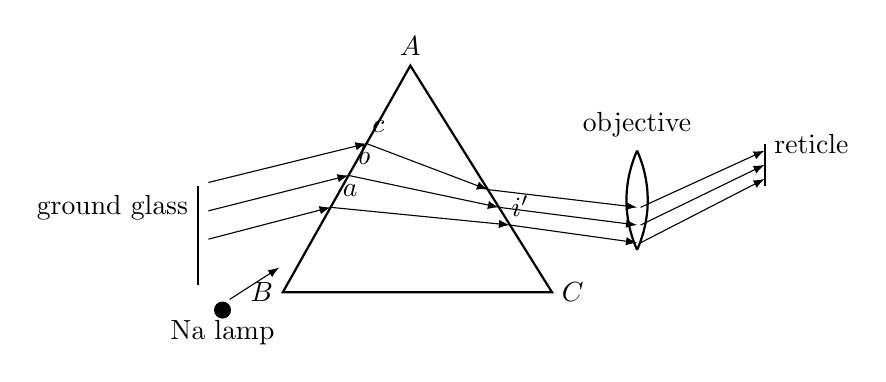
\begin{tikzpicture}[x=0.9cm,y=0.9cm,>=latex]
% prism
\coordinate (A) at (3.0,3.6);
\coordinate (B) at (1.2,0.4);
\coordinate (C) at (5.0,0.4);
\draw[thick] (A) -- (B) -- (C) -- cycle;
\node[above] at (A) {$A$};
\node[left] at (B) {$B$};
\node[right] at (C) {$C$};
% ground glass and sodium lamp
\draw[thick] (0.0,0.5) -- (0.0,1.9);
\node[left] at (0.0,1.6) {ground glass};
\fill (0.35,0.15) circle (0.12) node[below] {Na lamp};
\draw[->] (0.45,0.3) -- (1.15,0.75);
% rays a, b, c entering face AB
\draw[->] (0.15,1.15) -- (1.875,1.6);
\draw[->] (1.875,1.6) -- (4.406,1.35);
\draw[->] (4.406,1.35) -- (6.2,1.1);
\node[above] at (2.15,1.62) {$a$};
\draw[->] (0.15,1.55) -- (2.128,2.05);
\draw[->] (2.128,2.05) -- (4.25,1.6);
\draw[->] (4.25,1.6) -- (6.2,1.35);
\node[above] at (2.35,2.07) {$b$};
\draw[->] (0.15,1.95) -- (2.381,2.5);
\draw[->] (2.381,2.5) -- (4.094,1.85);
\draw[->] (4.094,1.85) -- (6.2,1.6);
\node[above] at (2.55,2.52) {$c$};
% objective and reticle
\draw[thick] (6.2,1.0) .. controls (6.4,1.45) and (6.4,1.95) .. (6.2,2.4);
\draw[thick] (6.2,1.0) .. controls (6.0,1.45) and (6.0,1.95) .. (6.2,2.4);
\node[above] at (6.2,2.45) {objective};
\draw[thick] (8.0,1.9) -- (8.0,2.5);
\node[right] at (8.0,2.5) {reticle};
% rays to the reticle
\draw[->] (6.25,1.1) -- (8.0,2.0);
\draw[->] (6.25,1.35) -- (8.0,2.2);
\draw[->] (6.25,1.6) -- (8.0,2.4);
\node at (4.55,1.62) {$i'$};
\end{tikzpicture}
\end{figbox}

\textbf{2.} The wavelength of sodium light is $\lambda=589.3\,\mathrm{nm}$. The scale division of the spectrometer is $30''$. With the spectrometer the apex angle of the prism was measured as $A=60\degree11'8''$, and the angle of emergence (minimum) as $i'=47\degree34'14''$. Substituting into the formula gives $n=1.7399$ (for a wavelength of $589.3\,\mathrm{nm}$). The apex angle $A$ and the minimum emergence angle $i'$ are both obtained by averaging several measurements.
